% ===========================
%       Chapter 1A.1
%     Chemistry of Life
%   Created by Michael Tang
%        2024.12.29
% ===========================

\subsubsection{Chemistry of Life}
\paragraph{\underline{Ionic Bonding} (离子键)}
\begin{itemize}
    \item \textbf{Definition:} Atoms transfer electrons to achieve a stable electron configuration, resulting in positively
    charged cations and negatively charged anions.
    \item \textbf{Key Properties:}
    \begin{itemize}
        \item High melting and boiling points.
        \item Solubility in polar solvents like water.
    \end{itemize}
    \item \textbf{Example:} \underline{Sodium} ($Na$ 钠) and \underline{chlorine} ($Cl$ 氯) form sodium chloride ($NaCl$ 氯).
    Sodium donates an electron to chlorine, forming a strong ionic bond.
    \begin{figure}[H]
        \centering
        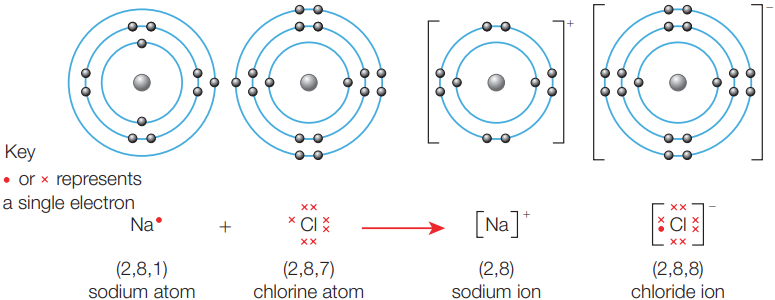
\includegraphics[scale=0.8]{Biology/1A/Images/1A-1-1.png}
        \caption{The formation of sodium chloride.}
    \end{figure}
\end{itemize}

\paragraph{Covalent Bonding}
\begin{itemize}
    \item \textbf{Definition:} Atoms shere electrons to achieve stability.
    \item \textbf{\underline{Polarity} (极性):} Unequal sharing of electrons leads to \underline{polar molecules} (极性分子 e.g.,
    water).
    \item \textbf{\underline{Dipoles} (偶极子):} Partial charges within the molecule, represented as $\delta^+$ (positive) and
    $\delta^-$ (negative).
    \begin{figure}[H]
        \centering
        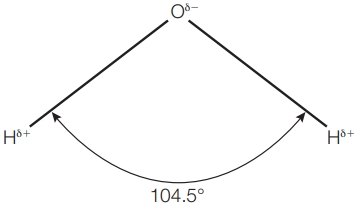
\includegraphics[scale=0.5]{Biology/1A/Images/1A-1-3.png}
        \caption{A model of a water molecule showing dipoles.}
    \end{figure}
    \item \textbf{Examples:} Formation of \underline{hydrogen} ($H_2$ 氢气) molecules and the formation of \underline{water}
    ($H_2O$ 水).
    \begin{figure}[H]
        \centering
        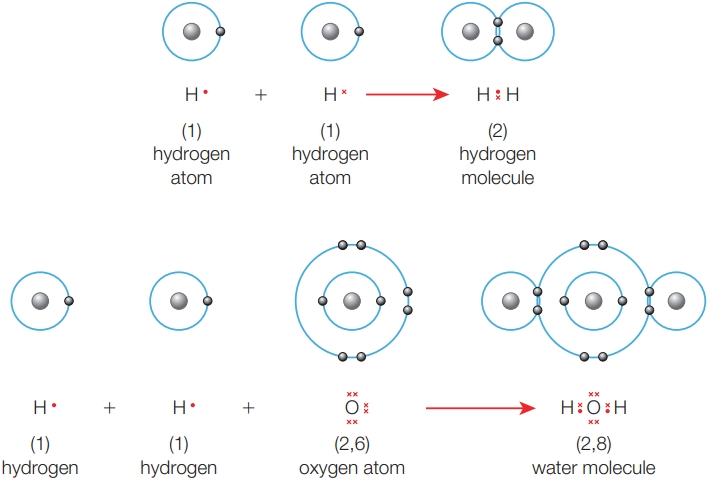
\includegraphics[scale=0.5]{Biology/1A/Images/1A-1-2.png}
        \caption{The formation of hydrogen molecules and water molecules are examples of covalent bonding.}
    \end{figure}
\end{itemize}

\paragraph{Chemistry of Water}
\begin{itemize}
    \item \textbf{Molecular Structure}
    \begin{itemize}
        \item \textbf{Polar Molecule:} Water ($H_2O$) has a bent structure with a partial charges (see figure 2.2) - oxygen is
        $\delta^-$, and hydrogen is $\delta^+$.
        \item \textbf{\underline{Hydrogen Bonding} (氢键):} Weak attractions between water molecules, providing
        \underline{cohesion} (凝聚力) and a relatively high boiling point.
        \begin{figure}[H]
            \centering
            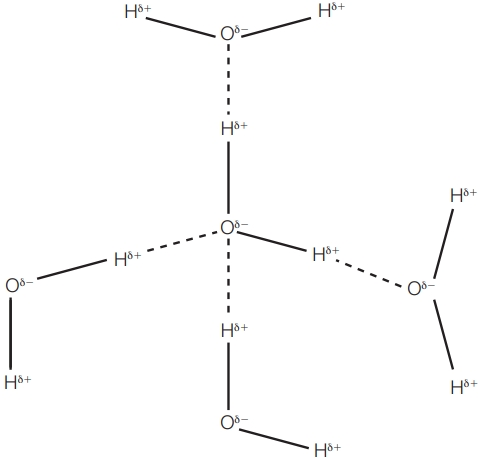
\includegraphics[scale=0.3]{Biology/1A/Images/1A-1-5.png}
            \caption{Hydrogen bonding in water molecules, based on attraction between positive and negative dipoles.}
        \end{figure}
    \end{itemize}
    \item \textbf{Unique Properties}
    \begin{itemize}
        \item \textbf{\underline{Solvent} (溶剂) Properties}
        \begin{itemize}
            \item Excellent solvent for ionic and polar \underline{substances} (物质).
            \begin{figure}[H]
                \centering
                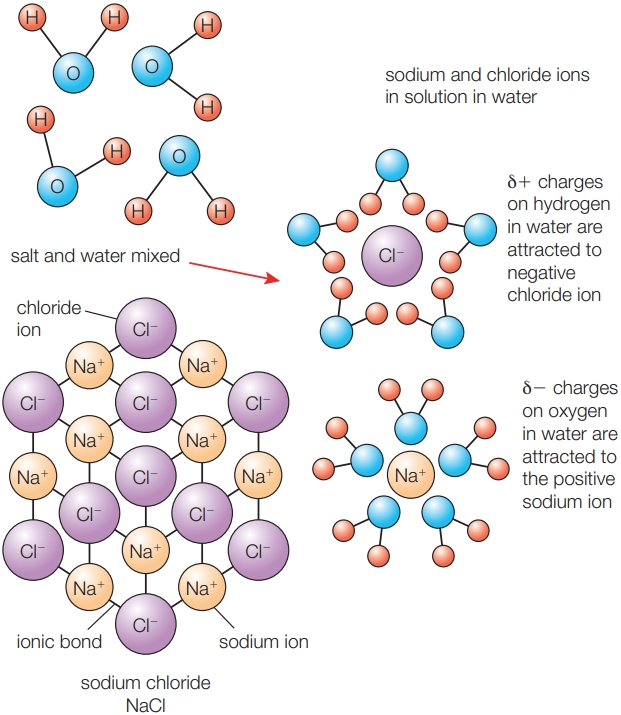
\includegraphics[scale=0.25]{Biology/1A/Images/1A-1-4.png}
                \caption{A model of sodium chloride dissolving in water as a result of the interactions between the charges on
                sodium and chloride ions and the dipoles of the water molecules.}
            \end{figure}
            \item \underline{Facilitates} (促进) \underline{biochemical} (生化) reactions in \underline{aqueous solutions} (水溶液).
        \end{itemize}
        \item \textbf{\underline{Thermal} (热) Stability}
        \begin{itemize}
            \item High specific \underline{heat capacity} \footnote{\textbf{Heat capacity: } Heat capacity refers to the amount of
            heat energy required to raise the temperature of a substance by one degree Celsius. It reflects the substance's
            ability to store \underline{thermal energy} (热能). $c$ is the symbol of heat capacity. The general formula of heat
            capacity is $c = \frac{Q}{m (t - t_0)} = \frac{Q}{m \Delta t}$. $\unit{J.kg^{-1}.K^{-1}}$ is the SI unit of heat
            capacity and $\frac{J}{(kg \cdot ^{\circ} C)}$ is the common unit.} (比热容) moderates temperature changes.
            \item Ice floats due to lower \underline{density} (密度) compared to liquid water, \underline{insulating} (隔热) the
            \underline{aquatic} (水生) life.
        \end{itemize}
        \item \textbf{\underline{Cohesion} (凝聚力) and \underline{Adhesion} (粘附力)}
        \begin{itemize}
            \item Enables water transport in plants.
            \item High surface tension due to hydrogen bonding.
        \end{itemize}
    \end{itemize}
\end{itemize}

\paragraph{Importance of Water}
\begin{itemize}
    \item \textbf{Biological Reactions:} All cellular reactions occur in an aqueous environment.
    \item \textbf{Transport Medium:} Dissolves and carries \underline{nutrients} (营养物质), gases, and \underline{waste products}
    (废物).
    \item \textbf{Habitat:} Provides a stable environment for \underline{diverse} (多样的) life forms.
    \item \textbf{Temperature Regulation:}
    \begin{itemize}
        \item \underline{Evaporation} (蒸发) cools organisms.
        \item High specific heat stability ecosystems.
    \end{itemize}
    \item \textbf{Structural Support:} \underline{Turgor pressure} \footnote{\textbf{Turgor pressure:} Turgor pressure is the
    pressure exerted by the water-filled \underline{vacuole} (液泡) against the cell wall in plant cells. It results from water
    entering the cell by \underline{osmosis} (渗透) and helps maintain the cell's \underline{rigidity} (刚性), supporting the
    plant's structure and preventing \underline{wilting} (枯萎).} (胀压) in plants depends on water.
\end{itemize}

\paragraph{Importance of \underline{Inorganic} (无机) Ions}
\begin{itemize}
    \item \textbf{Nitrate Ions ($NO_3^-$ 硝酸根离子):} Vital for DNA \footnote{\textbf{DNA (Deoxyribonucleic Acid 脱氧核糖核酸):} DNA
    is a molecule that carries the \underline{genetic instructions} (遗传信息) used in the growth, development, functioning, and
    reproduction of all living organisms. It consists of two strands forming a double \underline{helix} (螺旋), with each
    \underline{strand} (股) made up of \underline{nucleotide} (核苷酸) bases (adenine 腺嘌呤, thymine 胸腺嘧啶, cytosine 胞嘧啶,
    and guanine 鸟嘌呤). These bases pair specifically (A-T, C-G) and encode the instructions for \underline{synthesizing} (合成)
    proteins, which determine an organism's \underline{traits} (特征).} and \underline{protein synthesis} (蛋白质合成) in plants.
    \item \textbf{Phosphate Ions ($PO_4^{3-}$ 磷酸根离子):} Essential for ATP \footnote{\textbf{ATP (Adenosine Triphosphate
    腺嘌呤核苷三磷酸):} ATP is a molecule that acts as the primary energy carrier in cells. It consists of an \underline{adenosine
    molecule} (腺苷分子) bonded to three \underline{phosphate} (磷酸盐) groups. When ATP is broken down into ADP (adenosine
    diphosphate 二磷酸腺苷/核苷酸) and a phosphate group, energy is released to fuel cellular processes such as muscle contraction,
    active transport, and chemical synthesis.}, DNA \footnotemark[3], and RNA \footnote{\textbf{RNA (Ribonucleic Acid 核糖核酸):}
    RNA is a \underline{single-stranded nucleic acid} (单链核酸) that plays a crucial role in protein synthesis and gene
    expression. It is composed of \underline{ribose sugar} (核糖/单糖), phosphate groups, and four \underline{nitrogenous bases}
    (含氮碱基): adenine (A 腺嘌呤), uracil (U 尿嘧啶), cytosine (C 胞嘧啶), and guanine (G 鸟嘌呤). Unlike DNA, RNA contains uracil
    instead of thymine. Types of RNA include: mRNA \footnotemark[6] (messager RNA 信使核糖核酸), tRNA \footnotemark[7] (transfer
    RNA 转运核糖核酸), and rRNA \footnotemark[8] (ribosomal RNA 核糖体).}.
    \footnotetext[6]{\textbf{mRNA:} mRNA is a type of RNA that carries the genetic information from DNA in the cell nucleus to
    the \underline{ribosome} (核糖体), where it is used as a template for protein synthesis. It is transcribed from DNA and
    contains \underline{codons} \footnotemark[9] (密码子) that specify the \underline{amino acids} (氨基酸) to be incorporated
    into the protein.}
    \footnotetext[7]{\textbf{tRNA:} tRNA is a type of RNA that helps decode the genetic instructions in mRNA during protein
    synthesis. It carries specific amino acids to the ribosome, where it pairs its \underline{anticodon} \footnotemark[10]
    (反密码子) with the complementary codon on the mRNA sequence. This ensures that amino acids are added in the correct sequence
    to form a protein.}
    \footnotetext[8]{\textbf{rRNA:} rRNA is a type of RNA that is a key structural and functional component of ribosomes, the
    \underline{molecular machines} \footnotemark[11] (分子机器) that synthesize proteins. rRNA helps align mRNA and tRNA during
    protein synthesis and catalyzes the formation of \underline{peptide bonds} (肽键) between amino acids, facilitating the
    assembly of proteins.}
    \footnotetext[9]{\textbf{Codon:} A codon is a sequence of three nucleotide bases in mRNA that corresponds to a specific
    amino acid or a stop signal during protein synthesis. For example, the \underline{codon AUG} \footnotemark[12] (起始密码子)
    codes for the amino acid \underline{methionine} (蛋氨酸) and also serves as the start signal for translation.}
    \footnotetext[10]{\textbf{Anticodon:} An anticodon is a sequence of three nucleotide bases on a tRNA molecule that is
    complementary to a codon on the mRNA strand. During protein synthesis, the anticodon pairs with its corresponding codon,
    ensuring that the correct amino acid is added to the growing polypeptide chain.}
    \footnotetext[11]{\textbf{Molecular machines:} Molecular machines are complex biomolecules or assemblies of molecules that
    perform specific tasks within a cell, often converting energy into mechanical work. Examples include ribosomes for protein
    synthesis, ATP synthase for energy production, and \underline{motor proteins} \footnotemark[13] (马达蛋白) like
    \underline{kinesin} (驱动蛋白) for \underline{intracellular transport} (细胞内运输).}
    \footnotetext[12]{\textbf{Codon AUG:} The codon AUG serves two critical roles in protein synthesis: start codon, it signals
    the beginning of translation, indicating where the ribosome should start assembling the protein; and amino acid, AUG codes
    for the amino acid methionine (Met), which is often the first amino acid in newly synthesized proteins. This dual function
    makes AUG essential in the initiation of protein synthesis.}
    \footnotetext[13]{\textbf{Motor proteins:} Motor proteins are specialized molecular machines that convert chemical energy
    from ATP into mechanical work to perform cellular movements. They play key roles in intracellular transport, cell division,
    and structural support. Examples include: \underline{kinesin} (驱动蛋白), \underline{dynein} (动力蛋白), and \underline{myosin}
    (肌球蛋白).}
    \item \textbf{Sodium Ions ($Na^+$ 钠离子):} Critical in nerve impulses and secretory functions.
    \item \textbf{Magnesium Ions ($Mg^{2+}$ 镁离子):} Supports muscle contraction and structural roles in plants and animals.
    \item \textbf{Hydrogen Carbonate Ions ($HCO_3^-$ 碳酸氢根离子):} Maintains blood pH balance.
\end{itemize}
